% main.tex -- paper draft v3 (English, simple language). Compile: latexmk -pdf main.tex
% Numbers: paper_analysis/out/*.txt|csv, runs/odra_campaign/*/ (summaries), paper_draft/v3/szkic_pl.md.
% Figures: python -m paper_analysis.paper_figs_v3 --lang en
% Items marked \VERIFY must be checked before submission.
\documentclass[aps,pra,twocolumn,superscriptaddress,nofootinbib,10pt]{revtex4-2}
\usepackage[T1]{fontenc}
\usepackage[utf8]{inputenc}
\usepackage{amsmath,amssymb}
\usepackage{graphicx}
\usepackage{booktabs}
\usepackage{xcolor}
\usepackage[hidelinks]{hyperref}

\newcommand{\VERIFY}[1]{\textcolor{red}{[#1]}}
\newcommand{\ev}[1]{\langle #1\rangle}
\newcommand{\ket}[1]{|#1\rangle}
\newcommand{\Oid}{O_{\mathrm{id}}}
\newcommand{\ex}{$^{*}$}

\renewcommand{\topfraction}{0.95}
\renewcommand{\bottomfraction}{0.9}
\renewcommand{\textfraction}{0.05}
\renewcommand{\floatpagefraction}{0.8}
\renewcommand{\dbltopfraction}{0.95}
\renewcommand{\dblfloatpagefraction}{0.8}
\setcounter{dbltopnumber}{3}
\begin{document}

\title{Where error mitigation stops paying on a routed processor:\\
pre-registered hardware tests, mechanisms, and why classifier accuracy does not move}

\author{Karina Le\'skiewicz}
\affiliation{KN Axion, Wroc{\l}aw University of Science and Technology, Poland}

\date{\today}

\begin{abstract}
A quantum processor can only apply two-qubit gates between neighbouring qubits, so the
compiler adds gates that compute nothing but add noise. We ask how much of this overhead
error mitigation can absorb, and what it buys a quantum classifier. On the five-qubit IQM
ODRA~5 processor we compile one kind of classifier to 12--57 CZ gates, give every method the
same number of shots, compare it with a control of equal cost, and fix the tests before the
analysis. One simple picture explains the results: noise shrinks the output towards zero, and
mitigation works as long as this shrinking is the only damage and can be measured. The
shrinking grows mainly with circuit duration, and a simulator built from the device
calibration predicts it: inverting the predicted line, with no training shots on the
hardware, more than halves the error. Zero-noise extrapolation (ZNE) works only for the
shallowest circuit; beyond it, the noise-amplified circuits carry no signal and ZNE merely
rescales the output. Clifford data regression (CDR) pays much longer, and with Pauli twirling
its error stays low over the whole range, but its usual quality measure declares failure too
early. The error that remains after CDR grows with the number of CZ gates, is invisible to
the calibration model, and is removed by twirling. Two methods expected to help, variable-noise
CDR and dynamical decoupling, did not. Finally, mitigation can change a classifier decision
only near the decision boundary, where the noiseless classifier is itself guessing: it
restores the ideal circuit's decisions but leaves the accuracy unchanged.
\end{abstract}

\maketitle

% =========================================================================================
\section{Introduction}

A quantum classifier returns a decision: the class is the sign of a measured expectation
value $\ev{O}$~\cite{schuld2021,perezsalinas2020,bowles2024}. Error mitigation, however, is
almost always judged by how close it brings $\ev{O}$ to its ideal value~\cite{cai2023}. Work
on quantum machine learning under noise asks mostly whether models can be trained
\cite{wang2021nibp,wang2024em}, how to encode data robustly~\cite{larose2020}, or how to
train with noise in the loop~\cite{wang2022qnat}. We ask a simpler question. We have a
trained classifier and run it on hardware. Does mitigation change its decisions, and does it
pay at all at the cost the circuit has after compilation?

That cost comes from the hardware. Qubits are connected only to their neighbours, so the
compiler inserts SWAP gates, each made of three CZ gates. On our device the same kind of
classifier costs between 12 and 57 CZ gates, depending only on which qubits it entangles.
Theory says that the cost of any mitigation method grows exponentially with depth
\cite{takagi2022,quek2024}. It does not say at how many gates a given method stops paying on
a given device.

Three methods dominate in practice. Zero-noise extrapolation (ZNE) runs the circuit at
amplified noise and extrapolates to zero noise~\cite{temme2017,li2017,kandala2019,giurgica2020};
K\"oster and Mauerer showed that when the amplified circuits lose their signal, ZNE reduces to
rescaling a single measurement~\cite{koster2026}. Clifford data regression (CDR) learns a
straight line from noisy to ideal values on circuits whose ideal value can be computed
classically~\cite{czarnik2021}; variable-noise CDR (vnCDR) adds measurements at several noise
levels~\cite{lowe2021}. Pauli twirling turns part of the error into random noise that the
other methods handle better~\cite{wallman2016,hashim2021,kim2023}. Comparisons of these
methods come mostly from simulation~\cite{lowe2021,bultrini2023}; hardware studies either do
not resolve depth~\cite{russo2023} or check ZNE only where the answer can be computed
classically~\cite{kim2023}.

Four things are missing: a hardware measurement of how the gain of each method falls with
every added CZ gate, at equal cost and with a control that separates real extrapolation from
rescaling; an explanation of what breaks each method and whether a calibration model sees
it; tests fixed before the analysis~\cite{nosek2018}, without which a negative result is hard
to tell from a poor analysis; and a check of what mitigation does to the decisions of a
classifier, not only to $\ev{O}$.

We provide these on the IQM ODRA~5 processor. All results follow from one simple picture:
noise shrinks the output towards zero, $\ev{O}_{\rm meas}\approx s\,\Oid+c$, and mitigation
works as long as this shrinking is the only damage and can be measured. Our contributions:
\begin{enumerate}
\item \textbf{Decisions.} Mitigation changes a decision only near the decision boundary,
where the noiseless classifier is right in 44\% of cases (1300 hardware decisions). It
restores the ideal decisions without changing accuracy. An exact formula says when it would.
\item \textbf{The shrinking is predictable.} The retained signal $s$ falls mainly with circuit
duration and is predicted by a calibration-based simulator; inverting the predicted line
with no training shots more than halves the error. The prediction needs the circuit's schedule, not
per-qubit detail; a formula in gate counts fails.
\item \textbf{ZNE} is a real extrapolation only at 12 CZ; beyond that it is a rescaling,
and the model predicts its error without any fit.
\item \textbf{CDR} keeps an advantage up to about 63 CZ, while its fit quality $r^2$
declares failure much earlier; we show why.
\item \textbf{What lies beyond the shrinking} grows with CZ count, not duration, is invisible
to the calibration model, and is removed by twirling; it is not a fixed error of single CZ gates.
\item \textbf{Negative results} for vnCDR and dynamical decoupling in pre-registered tests.
\end{enumerate}

% =========================================================================================
\section{Setup}

\textbf{Device.} IQM ODRA~5 has five transmon qubits in a star: a central hub connected to
four outer qubits. Native gates are a single-qubit rotation PRX (20~ns) and CZ (60~ns).
During the experiments $T_1$ was 13--24~\textmu s and readout errors were 0.3--0.8\%
($0\to1$) and 2.5--5.1\% ($1\to0$). Every gate between outer qubits must pass through the
hub, so routing cost grows quickly and is easy to control. Access was unlimited.

\textbf{Classifier and ladder.} The classifier separates the two classes of the
\texttt{two\_curves} dataset~\cite{bowles2024}. It has 5 qubits, 3 layers and 55 weights;
data enter as rotation angles repeated in every layer. The output is the mean $\ev{Z}$ over
the five qubits and the decision is its sign. It is trained without noise and frozen. Four
entangling patterns give a ladder of 12, 30, 39 and 57 CZ gates after compilation (star,
linear, circular, all-to-all; noiseless test accuracy 0.73, 0.69, 0.68, 0.77). The task is
the same, but each rung is a separately trained circuit. Most experiments use the same 8 test
points, two from each quarter of the margin $|\Oid|$, the distance of the ideal output from
the decision boundary; one survey uses 100 points.

\textbf{Compilation.} Every circuit is compiled the same way (qubit 0 on the hub, fixed
seed, merged single-qubit rotations). All helper circuits for CDR and ZNE are built on the
compiled circuit, so they have exactly the same CZ gates in the same places as the target.

\textbf{CDR and twirling.} For each point we build 20 training circuits by replacing every
rotation angle of the compiled target with a nearby multiple of $\pi/2$. Such Clifford
circuits can be simulated efficiently at any size~\cite{gottesman1998,aaronson2004}, so their
ideal values are known. We fit $\Oid\approx a\,\ev{O}_{\rm meas}+b$ and apply it to the target.
Twirling wraps each CZ in a random pair of Pauli gates that cancels without noise; averaging
over such \emph{frames} turns part of the error into random noise. \emph{Native} twirling
wraps every physical CZ; \emph{logical} twirling wraps only the gates of the uncompiled
circuit, leaving routing gates bare. Every arm gets the same budget, $21\times6\times8192
\approx 10^6$ shots per point: six identical copies (untwirled control), six native frames,
six logical frames, or 120 different training circuits with one frame each (\emph{spread}).

\textbf{ZNE and its control.} ZNE replaces the circuit $U$ by $U(U^\dagger U)^k$ to amplify
noise by $\lambda=3,5$ and extrapolates with Richardson's formula, without clipping (8192 shots
per scale). The \emph{garbage} control uses $U(V^\dagger U)^k$, where $V$ has the same CZ
gates but random rotations: the noise is the same, but the amplified circuits know nothing
about the answer. If ZNE does no better than garbage, its gain is not extrapolation
\cite{koster2026}. Readout errors are also corrected offline, at no shot cost.

\textbf{Duration versus gates.} Into the 12-CZ circuit we insert 6, 12 or 20 pairs of CZ
gates that cancel (24, 36, 52 CZ, same function) or a wait of exactly the same length (still
12 CZ). Durations (0.8--3.2~\textmu s) come from the gate schedule.

\textbf{Further experiments.} \emph{vnCDR}: on the 12-CZ circuit every circuit is measured at
three interleaved levels (as is, $+12$ CZ pairs, $+$matched wait), with the same total shots
as CDR. \emph{DD}: CDR on the 12- and 39-CZ circuits with and without the vendor's dynamical
decoupling, interleaved copy by copy. \emph{Decision survey}: 13 circuit variants $\times$
100 points, unmitigated only, plus $\ket{00000}$ and $\ket{11111}$ to measure readout.

\textbf{Calibration simulator.} A noise model built from the same night's calibration data
($T_1$, $T_2$, gate fidelities, readout errors) runs through exactly the same code as the
hardware. We also test whether a fixed over-rotation by an angle $\theta$ on every CZ
reproduces the hardware.

\textbf{Statistics and pre-registration.} The main measure is the error of one point,
$|\ev{O}_{\rm mit}-\Oid|$. Methods are compared in pairs on the same points with the Wilcoxon
test~\cite{wilcoxon1945} and the geometric mean of the error ratio. The analysis plan and code
were committed and tagged before any error was computed, but after the ladder measurements had
started~\cite{nosek2018}. The main hypotheses were: twirling lowers the CDR error (H1), native
twirling is no worse than logical (H3), spread beats twirling (H6), more CZ at fixed duration
raises the error (H7a), and longer duration at fixed gates raises the error (H7b), with Holm
correction~\cite{holm1979}. vnCDR and DD each had one hypothesis fixed before measurement.
Everything else is exploratory, marked \ex, with uncorrected $p$-values.

% =========================================================================================
\section{The contraction model}

For a given circuit and input $x$ we write
\begin{equation}
\ev{O}_{\rm meas}(x)= s\,\Oid(x)+c+r(x). \label{eq:model}
\end{equation}
The \emph{retention} $s\in(0,1]$ is the fraction of the output that survives the noise. It is
the same for all inputs and for circuits with the same gates. The offset $c$ is small and comes
mostly from readout. The residual $r(x)$ is everything the line does not describe. We call
$s\Oid+c$ the \emph{contraction}: noise mixes the state with a random one, whose $\ev{Z}$ is
zero, so the output shrinks towards zero. If $r=0$, mitigation is just
$\Oid=(\ev{O}_{\rm meas}-c)/s$, and every method is a different way of estimating $s$ and $c$.
That depolarizing noise rescales the output is known~\cite{vovrosh2021,urbanek2021}, and the
line is the core of CDR~\cite{czarnik2021}. The model is a first-order description, not a
derivation. Its use here is that one measured number, $s$, predicts where and why each method
fails.

% =========================================================================================
\section{Results}

\subsection{Noise shrinks the output, and the shrinking is predictable}

In every circuit variant the 100 survey points lie on a line (Fig.~\ref{fig:contraction}a).
Its slope $s$ falls from 0.85 at 12 CZ to 0.51, 0.30 and 0.24 at 30, 39 and 57 CZ\ex. Readout
adds $c\approx+0.03$.

The shrinking depends mainly on duration (Fig.~\ref{fig:contraction}b). Over the 13 variants,
duration alone explains 81\% of the variation of $\log s$, CZ count 74\%\ex. At equal duration,
CZ pairs shrink the output slightly more than waiting ($s=0.67,0.56,0.42$ vs.\ $0.75,0.64,0.53$),
so CZ gates add their part, but time dominates. The pre-registered test agrees: at fixed gates
each microsecond raises the unmitigated error 1.43-fold (H7b, Table~\ref{tab:p5}), our one
hypothesis confirmed after correction. The effect of CZ count at fixed duration is unresolved
(H7a).

The calibration simulator predicts the unmitigated output: the hardware error is 1.04 times
the model's, and over the 1300 survey values the correlation is 0.984\ex. Its slope $s$
matches the hardware within about 0.05 on the ladder and with added waiting, but it is too high
when CZ pairs are added (0.63 vs.\ 0.48 at 36 CZ, 0.54 vs.\ 0.41 at 52 CZ).

\textbf{Inverting the predicted line.}\ex\ Since the simulator knows $s$ and $c$, we can mitigate
without any training shots on the hardware: simulate the same 20 training circuits, fit the
line in simulation, and apply it to the hardware output. Over 112 point--variant pairs this
lowers the error in 85 cases (error ratio 0.41, $p=2\times10^{-10}$;
Fig.~\ref{fig:free}). It comes close to hardware CDR (ratio 1.15, $p=0.23$, 54 of 112 wins) at
about $1/21$ of its shots, and beats untwirled CDR on the deepest routed rungs (0.064 vs.\ 0.076
at 30 CZ, 0.092 vs.\ 0.152 at 57 CZ). It loses where CZ pairs were added, exactly where the
simulator overestimates $s$. Twirled CDR remains best (ratio 1.48 against it, $p=0.16$).

\textbf{What makes the prediction work?}\ex\ Two variants answer this (Table~\ref{tab:source}).
Giving every qubit the average $T_1$, $T_2$, gate and readout errors changes nothing (error ratio
0.95 against the full simulator, $p=0.07$). Replacing the simulator by a three-parameter formula in
CZ count, duration and PRX count, fitted to the night's hardware training circuits, does much worse:
1.83 times CDR's error ($p=10^{-4}$). The accuracy thus comes from simulating the actual circuit,
which qubits wait while others work and for how long, and not from per-qubit detail or from gate
counts. This also explains why an earlier attempt to invert such a count formula failed.

\begin{table}[b]
\caption{Where the line comes from.\ex\ Error ratio against hardware CDR (geometric mean) and wins
against the raw output, 112 point--variant pairs. Lines are fitted per point.}
\label{tab:source}
\begin{ruledtabular}
\begin{tabular}{lcc}
source of the line & vs.\ CDR ($p$) & beats raw \\
\hline
count formula (CZ, $t$, PRX) & 1.83 ($10^{-4}$) & 68/112 \\
full calibration simulator & 1.15 (0.23) & 85/112 \\
simulator, all qubits averaged & 1.09 (0.40) & 88/112 \\
\end{tabular}
\end{ruledtabular}
\end{table}

\begin{figure*}[!tbp]
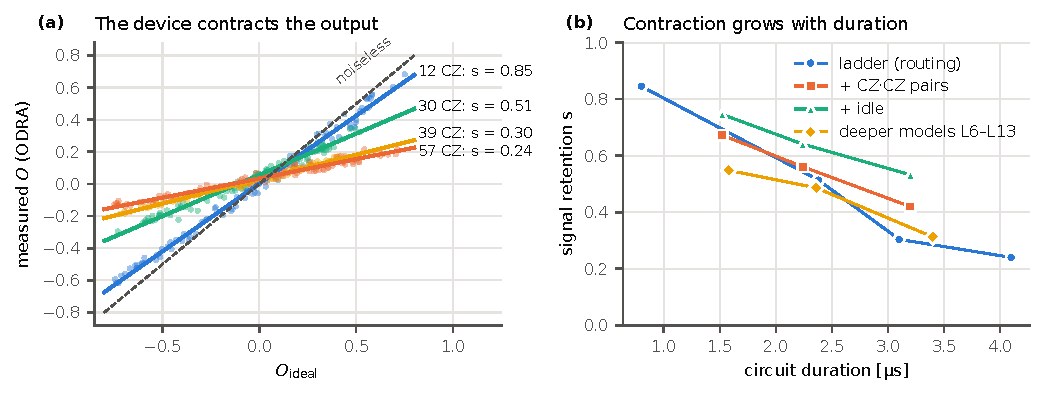
\includegraphics[width=0.8\textwidth]{figs/fig1_contraction.pdf}
\caption{The device as a contraction (decision survey). (a) Output measured on ODRA against
the ideal output, 100 points per rung; lines are fits, $s$ is the slope. (b) Retention $s$
against circuit duration for 13 variants: the ladder, the 12-CZ circuit with added CZ pairs,
the same circuit with an equally long wait, and deeper models.}
\label{fig:contraction}
\end{figure*}

\begin{figure*}[!tbp]
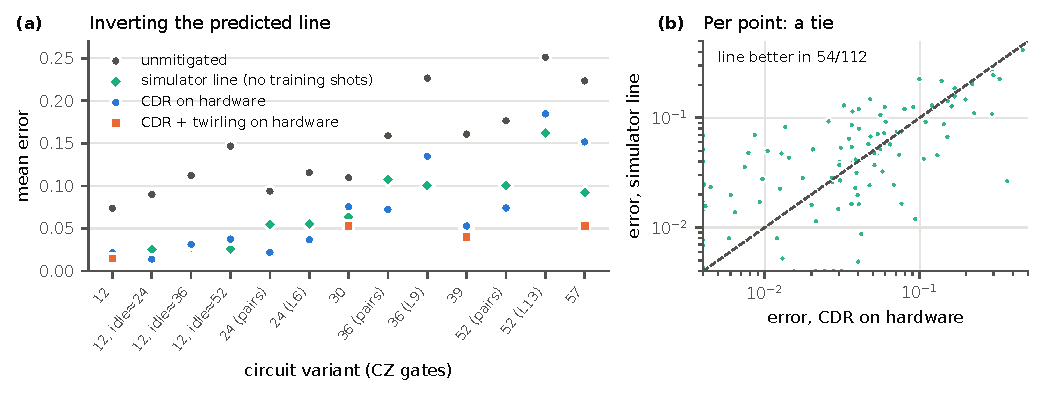
\includegraphics[width=0.8\textwidth]{figs/fig_free_mitigation.pdf}
\caption{Inverting the line predicted by the calibration simulator, with no training shots on
the hardware.\ex\ (a) Mean error per circuit variant. (b) Error per point against hardware CDR;
the dashed line marks equal error.}
\label{fig:free}
\end{figure*}

\subsection{ZNE needs signal in the amplified circuits}

If every fold shrinks the output by the same factor, the amplified circuits keep $s^3$ and
$s^5$ of the signal. At 12 CZ that is 0.61 and 0.44; at 39 CZ, 0.03 and 0.002.

\begin{table}[b]
\caption{Mean error on the ladder (8 points). Garbage: ZNE control of equal cost.
Sim.\ line: inverting the simulator-predicted line\ex.}
\label{tab:ladder}
\begin{ruledtabular}
\begin{tabular}{lcccccc}
CZ & raw & ZNE & garbage & CDR & CDR+tw. & sim.\ line \\
\hline
12 & 0.074 & 0.045 & 0.137 & 0.022 & 0.015 & 0.023 \\
30 & 0.110 & 0.064 & 0.068 & 0.076 & 0.053 & 0.064 \\
39 & 0.161 & 0.112 & 0.103 & 0.053 & 0.040 & 0.050 \\
57 & 0.223 & 0.170 & 0.161 & 0.152 & 0.053 & 0.092 \\
\end{tabular}
\end{ruledtabular}
\end{table}

At 12 CZ, ZNE extrapolates: it beats garbage at 7 of 8 points ($p=0.012$) and its curves point
towards the ideal values (Fig.~\ref{fig:zne}a). It does not beat the raw output ($p=0.47$),
because folding amplifies gate noise but not readout; after readout correction its error drops
to 0.016\ex. From 30 CZ on, ZNE equals garbage (Table~\ref{tab:ladder}); at 39 CZ it is better
at only 2 of 8 points ($p=0.84$). At $\lambda=5$ all points give the same value although their
ideal values range from $-0.43$ to $+0.17$ (Fig.~\ref{fig:zne}b). Richardson's formula then
becomes $\tfrac{15}{8}E_1-\tfrac{7}{8}f$~\cite{koster2026}: the output times 1.9, minus the
background $f$. This partly undoes the shrinking, so ZNE beats raw at 39 CZ (8 of 8), but the
garbage control does the same. The pre-registered ZNE criterion (H4) fails at every rung.

The model predicts the size of this effect. With retention $s^\lambda$, Richardson returns
$g(s)\Oid$ with $g(s)=\tfrac{15}{8}s-\tfrac54 s^3+\tfrac38 s^5$, and the ratio of ZNE to raw
error is $|1-g(s)|/(1-s)$. With $s$ measured independently, this gives 0.67 and 0.75 at 39 and
57 CZ against measured 0.70 and 0.76\ex. At 12 and 30 CZ the measured ratio is worse (0.61,
0.58 vs.\ predicted 0.05, 0.40) because the readout offset, which folding does not amplify,
dominates there. At 39 CZ ZNE multiplies by 1.9 where $1/s\approx3.3$ is needed.

The pre-registered diagnostics missed the collapse (signal-to-noise against zero 4.1 at 39 CZ,
above the threshold of 2); measured against the garbage background it is 0.8, against 11.8 at
12 CZ. A second control, identity folding, is invalid on hardware: its output drifts towards
$+1$ as qubits relax to $\ket{0}$, which the simulator reproduces and which vanishes for
$T_1\to\infty$.

\begin{figure*}[!tbp]
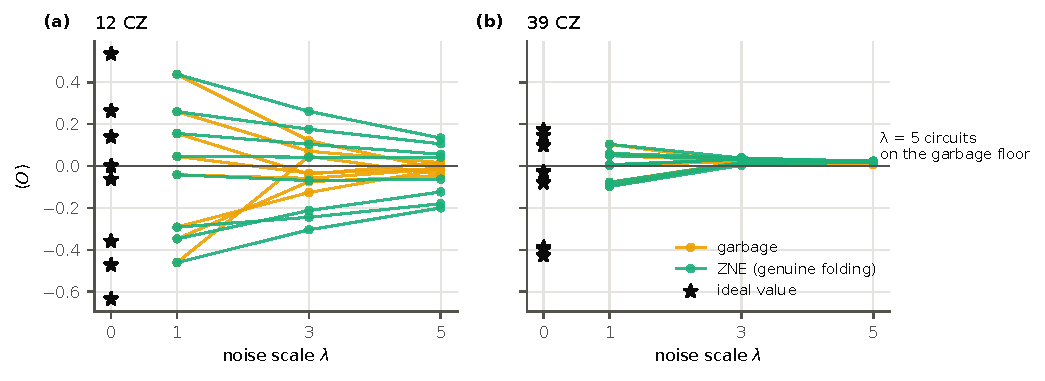
\includegraphics[width=0.8\textwidth]{figs/fig2_zne_collapse.pdf}
\caption{$\ev{O}$ against noise scale $\lambda$ for the 8 points: ZNE and the garbage control
with the same CZ gates; stars are ideal values. (a) 12 CZ. (b) 39 CZ: at $\lambda=3,5$ both
give the same value.}
\label{fig:zne}
\end{figure*}

\subsection{CDR learns the line and pays while the line holds}

CDR does directly what Fig.~\ref{fig:contraction} suggests. It needs no signal at amplified
noise, only a line that holds. Without twirling it beats the raw output on every rung (6/8,
6/8, 7/8, 5/8 points), but its advantage falls by about 25\% per 10 CZ over 15 variants and is
extrapolated to vanish near 63 CZ (95\% interval 50--79; Fig.~\ref{fig:cdr}a)\ex.

The fit quality $r^2$ falls much faster: it is 0.35 at 57 CZ, where CDR is still 1.5 times
better than raw (Fig.~\ref{fig:cdr}b). The threshold $r^2=0.8$ we used earlier would have
declared CDR broken at about 30 CZ. The model shows why. On the training circuits
\begin{equation}
r^2\approx\frac{s^2\,\mathrm{Var}(\Oid)}{s^2\,\mathrm{Var}(\Oid)+\mathrm{Var}(r)+\sigma^2_{\rm shot}},
\end{equation}
so $r^2$ falls when $s$ falls even if the residual does not change: the signal becomes small
next to the noise, while the line is still right on average. At 39 CZ, 78--85\% of training
circuits also have ideal value 0, which lowers $\mathrm{Var}(\Oid)$. A better criterion is
simple: CDR stops paying when it no longer beats the raw output or a control of equal cost.
Leave-one-out error on the training circuits predicts the mean CDR error per rung well (median
ratio 1.02)\ex, but deciding per point whether to use CDR is worse than always using it.

\begin{figure*}[!tbp]
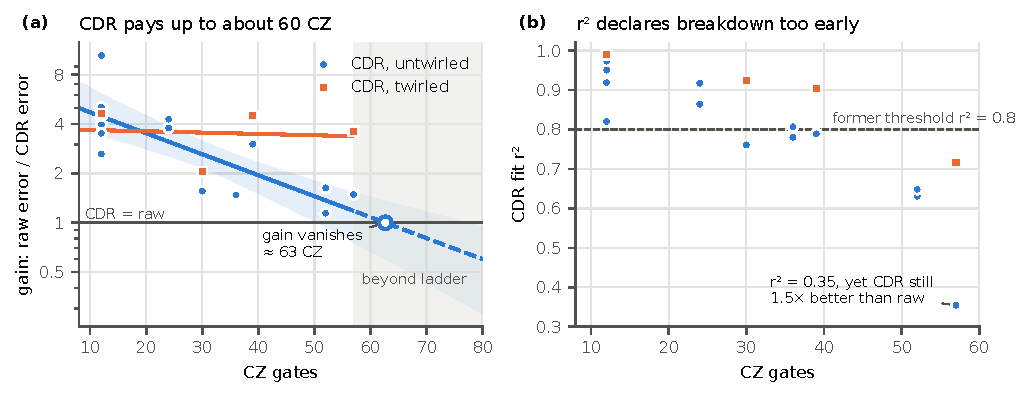
\includegraphics[width=0.8\textwidth]{figs/fig3_cdr_frontier.pdf}
\caption{(a) How many times CDR beats the raw output, against CZ count (log scale); line: fit
with 95\% band; dashed: extrapolation; circle: break-even. (b) CDR fit $r^2$ on the same
variants; dashed: the former threshold 0.8.}
\label{fig:cdr}
\end{figure*}

\subsection{What lies beyond the contraction}

The duration experiment separates time from gates on one circuit (Fig.~\ref{fig:p5},
Table~\ref{tab:p5}). The raw error grows similarly with CZ pairs and with waiting. After CDR it
is different: waiting leaves almost no error (0.014--0.037), CZ pairs do (0.072--0.074 at 36
and 52 CZ), and the error after CDR grows 1.34-fold per 10 CZ but not significantly with time.
The time-driven shrinking is shared by training and target circuits, so the line learns it; the
CZ-linked part transfers worse from Clifford circuits. Results hold when variants affected by a
calibration change are removed.

\begin{table}[t]
\caption{Duration experiment (56 measurements, 8 points, one level per point). $p$ from a
$t(7)$ reference and an exact wild-cluster bootstrap.}
\label{tab:p5}
\begin{ruledtabular}
\begin{tabular}{llccc}
error & added & factor & 95\% CI & $p$ ($t$/boot.) \\
\hline
raw & $+10$ CZ (fixed $t$) & 0.96 & 0.74--1.24 & 0.69/0.68 \\
raw & $+1$\,\textmu s (fixed gates) & \textbf{1.43} & 1.27--1.61 & $2\!\cdot\!10^{-4}$/0.008 \\
CDR & $+10$ CZ & \textbf{1.34} & 1.07--1.67 & 0.018/0.016 \\
CDR & $+1$\,\textmu s & 1.32 & 0.69--2.53 & 0.35/0.31 \\
\end{tabular}
\end{ruledtabular}
\end{table}

The calibration model does not see this residual. It underestimates the untwirled CDR error
1.88-fold (Fig.~\ref{fig:twirl}a)\ex, and the excess appears with CZ pairs ($+0.037$) but not with
waiting ($+0.006$, $p=0.0003$)\ex. It is not a fixed error of each CZ: adding an over-rotation
$\theta$ to every CZ does not reproduce the hardware for any $\theta\le0.15$ (at 57 CZ the model
gives $r^2=0.89$--$0.94$, the hardware 0.66), and larger $\theta$ breaks rungs that already fit.

\begin{figure*}[!tbp]
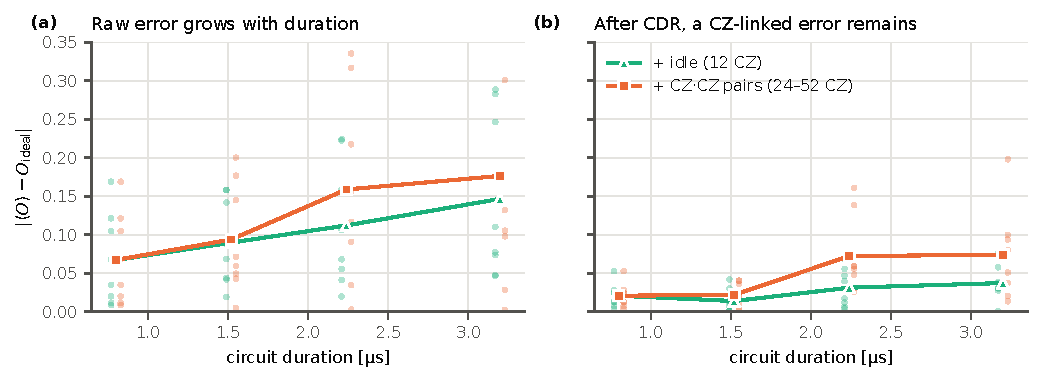
\includegraphics[width=0.8\textwidth]{figs/fig4_duration_vs_cz.pdf}
\caption{Duration experiment: the 12-CZ circuit with added CZ pairs or an equally long wait,
against duration. (a) Raw error. (b) Error after CDR. Lines join means; light dots are points.}
\label{fig:p5}
\end{figure*}

\subsection{Twirling restores the line}

With twirling the CDR error is 0.015, 0.053, 0.040 and 0.053 at 12, 30, 39 and 57 CZ, and its
advantage stays at 3.6--4.6 without falling with CZ count (Fig.~\ref{fig:cdr}a). $r^2$ rises
(0.35 to 0.72 at 57 CZ) and the calibration model agrees with the hardware again (ratio 0.86).
Twirling restores exactly what CDR needs. The pre-registered test did not confirm it: twirling
lowered the CDR error in 20 of 32 pairs ($p=0.09$; 0.37 after Holm). The gain is small at
shallow depth, and the output varies between frames 10--30 times more than shot noise\ex, so
with six frames the frame count, not the shot count, limits twirling.

Twirling routing gates adds nothing\ex\ (Fig.~\ref{fig:twirl}b). At 30 CZ native twirling wraps
30 gates and logical only 12, yet their errors are 0.036 and 0.029; at 12 CZ, where both do the
same thing physically, they differ by a similar amount (0.031 vs.\ 0.019). Frame variance is
the same in both. (The pre-registered H3 cannot be interpreted, because these arms shared one
training set across points.) Spreading the budget over more training circuits (H6) does not
help ($p=0.55$). Three independent observations thus agree: the residual is tied to CZ gates and
routing, but it is not a fixed error of single gates.

\begin{figure*}[!tbp]
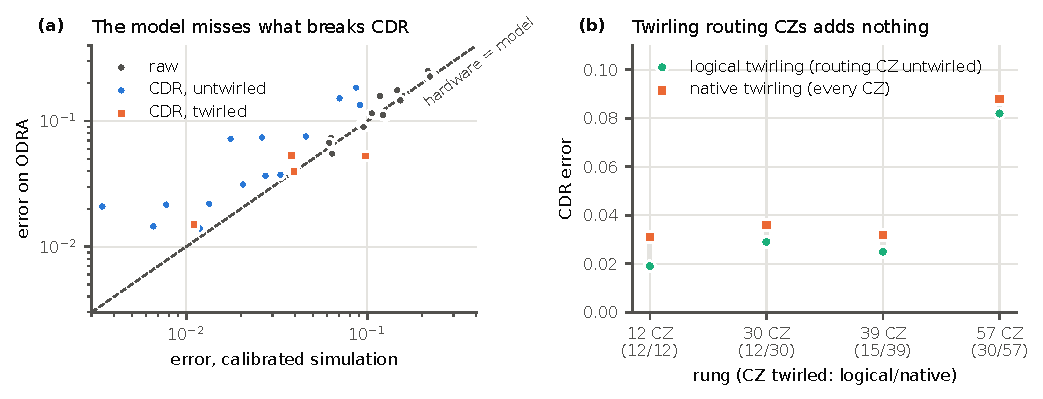
\includegraphics[width=0.8\textwidth]{figs/fig5_beyond_contraction.pdf}
\caption{(a) Error on ODRA against error in the simulation with the same night's calibration,
per rung and method; dashed: equality.\ex\ (b) CDR error with logical and native twirling.\ex}
\label{fig:twirl}
\end{figure*}

\subsection{More noise information does not help}

vnCDR did not beat CDR at equal shots: error 0.017 vs.\ 0.015, better at 4 of 8 points
($p=0.63$), although the simulation of the same experiment predicted half the error. DD did not
help either: CDR error 0.115 with DD and 0.063 without, better at 4 of 16 pairs ($p=0.065$, so
``no difference detected'' as pre-registered). Its direction is clear: DD worsened the raw output
at 12 CZ at 8 of 8 points (0.047 to 0.125)\ex\ and lowered the CDR $r^2$ on both rungs (0.97 to
0.87, 0.62 to 0.34)\ex. The arms were interleaved under one calibration, so drift cannot explain it.

\subsection{Classifier decisions}

A decision is the sign of the output. The contraction does not change signs, so noise flips a
decision only when $|\Oid|<|c|/s$, near the boundary. Linear mitigation $a\ev{O}_{\rm meas}+b$ only
moves the threshold from 0 to $-b/a$; this covers CDR, readout correction and ZNE once it has
collapsed. When mitigation changes a decision, exactly one of the two decisions is right, so
\begin{equation}
\Delta\mathrm{acc}=P(\text{change})\,(2q-1), \label{eq:dacc}
\end{equation}
where $q$ is the fraction of changed decisions that mitigation gets right. When mitigation
restores the ideal decision, $q$ is the accuracy of the noiseless classifier near the boundary.

On hardware, noise flipped 91 of 1300 survey decisions (7\%), with median margin 0.053 against
0.331 for all points (Fig.~\ref{fig:dec}a). At these points the noiseless classifier is right in
only 40 of 91 cases, 44\% (Fig.~\ref{fig:dec}b), so noise did not lower the accuracy (0.720 raw,
0.712 ideal). In simulation on three datasets\ex, CDR restores the ideal decision 132 times and
breaks it 32 times ($p=10^{-15}$), yet accuracy stays at 0.735 raw, 0.727 after CDR, 0.731
ideal. Eq.~\eqref{eq:dacc} gives exactly this: 164 changes, 74 right, $\Delta\mathrm{acc}=-0.008$.
The noiseless accuracy rises from about 0.5 near the boundary to 0.92 far from it, and noise
flips decisions only where it is about 0.5.

\begin{figure*}[!tbp]
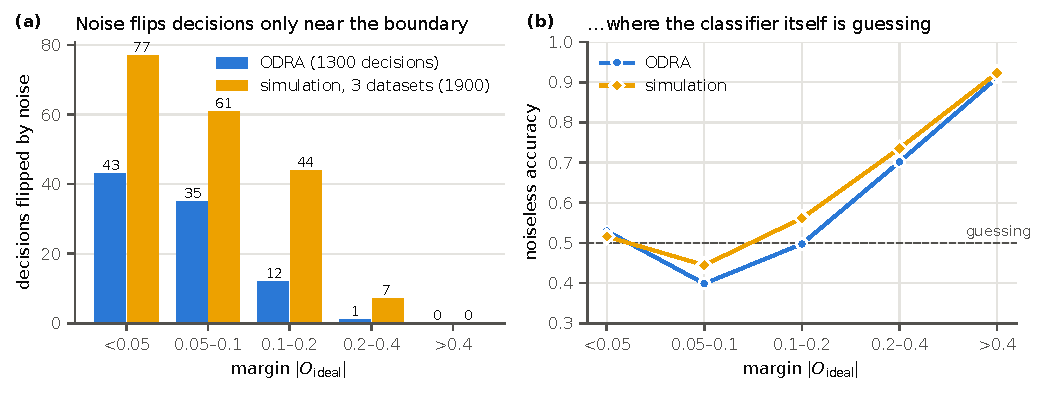
\includegraphics[width=0.8\textwidth]{figs/fig6_decisions.pdf}
\caption{(a) Decisions flipped by noise, by margin $|\Oid|$: ODRA (1300 decisions) and
simulation (three datasets). (b) Noiseless accuracy in the same bins; dashed: guessing.}
\label{fig:dec}
\end{figure*}

% =========================================================================================
\section{Why the methods behave as they do}

\textbf{Why the simulator line works.} Most of the damage on this device is the contraction,
and the contraction comes from incoherent processes: relaxation and dephasing during the
circuit, gate infidelity and readout. These are exactly what the calibration measures, qubit by
qubit and gate by gate. The simulator only adds them up along the real schedule, which is why
$s$ tracks duration and why the predicted $s$ is within about 0.05 of the measured one. The
schedule is what matters: averaging the qubits costs nothing, while reducing the circuit to its gate
counts loses most of the accuracy (Table~\ref{tab:source}).
Inverting the line then removes the contraction and leaves only $r/s$. The simulator line also
avoids two problems of CDR on hardware. Its line is not blurred by shot noise in the training
data, and it is not biased by the residual $r$, which differs between Clifford training circuits
(about half the PRX gates, shorter, often ideal value 0) and the target. This is why it beats
untwirled CDR on routed rungs. It loses where $r$ is large and the calibration does not know it,
with added CZ pairs, where it overestimates $s$.

\textbf{Why ZNE fails.} ZNE must measure the output at $s^3$ and $s^5$. A single 8192-shot value
has a standard error of about 0.005. At 12 CZ the $\lambda=5$ output is still about 0.11, far
above it; at 39 CZ the signal left at $\lambda=5$ ($s^5|\Oid|\approx0.0005$) is ten times below
it, so the amplified circuits return only the background. Folding also leaves readout untouched,
so the offset $c$ survives even when extrapolation works.

\textbf{Why untwirled CDR weakens.} CDR assumes that training circuits and target share one line.
On hardware the residual $r$ is circuit-specific and grows with CZ gates, so the training points
scatter around the line and the line learned from them is biased for the target. As $s$ shrinks,
the same scatter weighs more, which is also what $r^2$ reports.

\textbf{Why twirling helps.} Twirling averages structured errors into random Pauli noise, which
acts like further contraction. It moves damage from $r$ into $s$: $s$ drops a little, but the
line holds again and is the same for training and target circuits. That is why the calibration
model, which has only random noise, fits twirled data.

\textbf{Why vnCDR and DD fail.} vnCDR adds measurements at 36 CZ, where $s\approx0.5$, so it
inherits part of ZNE's problem and fits more parameters from the same 20 circuits. DD adds
pulses whose own errors enlarge $r$; it lowered $r^2$ on both rungs.

\textbf{Why decisions do not move.} The contraction preserves signs, and linear mitigation only
moves a threshold. Both act only near the boundary, where the classifier is guessing.

% =========================================================================================
\section{Discussion}

\textbf{One model instead of a list of failures.} Without the model, our results are a list:
ZNE fails, $r^2$ falls, twirling helps, DD hurts, accuracy does not move. With it, they follow from
one measured number, $s$, and one residual, $r$, and can be checked before spending hardware time.

\textbf{CZ count is not the whole cost.} The contraction, which mitigation can undo, follows
duration; the residual, which it cannot, follows CZ count. The same gate count can therefore mean
different costs, and a formula in gate counts and duration predicts the contraction much worse than a
simulation of the actual schedule (Table~\ref{tab:source}). Earlier, less controlled measurements on two larger IQM lattices (Garnet, 20
qubits; Emerald, 54 qubits) showed the same shape of CDR degradation at about three times more CZ
gates than on the star, but they did not meet the standards of this work and are only a hint.
Studies should report circuit duration next to gate count.

\textbf{What the residual is.} It grows with CZ gates, is absent from the calibration model, is
removed by twirling and is not a fixed error of single gates. Mechanisms that act more strongly in
routed circuits fit these facts: crosstalk from a running gate onto waiting neighbours (routing
through the hub creates many such moments), leakage out of the qubit subspace, correlated errors
within the three CZ gates of a SWAP, and drift between calibration and measurement. Similar causes
were reported for a 20-qubit IQM device~\cite{iqm20bench}. We do not decide which dominates.

\textbf{For machine learning.} Eq.~\eqref{eq:dacc} changes the question from ``is this method
good'' to ``is my classifier right near its boundary''. Usually it is not, because the points near
the boundary are exactly the ones it separates worst. Mitigation can help when noise is strong
enough to flip points the classifier knows well, which matches our earlier observation on the
Banknote dataset, where mitigation raised accuracy only at high routing cost. For classification,
improving the margin, e.g.\ by robust encodings~\cite{larose2020}, is a better investment.
Mitigation matters where the value itself matters: probabilities, confidence, kernel values,
energies.

\textbf{A simple rule.} (1) Estimate $s$ for your circuit from a few Clifford circuits or from a
calibration simulator. (2) Use ZNE only if $s^3$ (and $s^5$) clearly exceed the shot noise.
(3) Use CDR with twirling at higher cost, and judge it against the raw output or a control of equal
cost, not by $r^2$. (4) Try the simulator line first: it is free and often close to CDR.
(5) For classification, first check how often the noiseless classifier is right near its boundary.

\textbf{Why the negative results count.} The tests were fixed before the analysis; the same
pipeline detects effects when they exist (CDR beats raw in 27 of 32 twirled pairs,
$p=1.6\times10^{-5}$; duration $p=2\times10^{-4}$); the garbage control shows that ZNE's gain is
apparent; and simulation predicted that vnCDR would help. The model also says why each result is
negative. Only the twirling test is weak: the trend is clear, but 8 points and 6 frames are too few.

% =========================================================================================
\section{Limitations}

All results come from one five-qubit star device; we do not know whether ``duration drives the
contraction, CZ gates drive the residual'' holds on other topologies. Main comparisons use 8 points
per rung, the same in every experiment, and the 100 survey points are reused across 13 variants.
Ladder rungs are different circuits, so gate count is tied to function there; the duration
experiment separates them for one circuit only. The calibration changed while the 30- and 57-CZ
rungs were measured, and some of those jobs interleaved with the survey; we detect recalibrations,
not drift between them, and a sensitivity analysis for 57 CZ is still due. The plan was fixed before
the analysis but after the ladder measurements began, and many analyses are exploratory. The model
is approximate (one $s$ for all inputs, constant $c$, retention $s^\lambda$), and durations are
computed, not measured. The over-rotation fit used older September twirling data. ZNE was tested
only with Richardson extrapolation at scales 1, 3, 5, DD only in the vendor's version, and PEC not
at all. The simulator line and the comparison of line sources are exploratory and were not
pre-registered; the 112 pairs come from 8 inputs. The simulated decision analysis uses a model without $r$,
so CDR looks too good there; the key fact, noiseless accuracy near the boundary, comes from
hardware. Six twirling frames limit the twirling test.

\section{Future work}

Extend the ladder beyond 57 CZ to measure, not extrapolate, where CDR stops paying. Repeat the
protocol on larger devices with other topologies. Identify the residual: measure the effect of a gate
on waiting neighbours, detect leakage, insert CZ pairs on edges with different numbers of neighbours,
and twirl only routing gates. Test the simulator line in a pre-registered experiment, against CDR,
with fresh calibrations and with averaged device numbers only, and ZNE with scales chosen so that $s^\lambda$ stays measurable.
Use more twirling frames and build CDR error bars that include frame variance. Test
Eq.~\eqref{eq:dacc} on classifiers with large margins and on tasks where the value matters.

\section*{Data and code}
All circuits, raw counts, calibration data, manifests, pre-registrations and analysis scripts are
in the project repository \VERIFY{add public URL / DOI}.

\begin{acknowledgments}
\VERIFY{Acknowledgments: KN Axion, IQM / ODRA access.}
\end{acknowledgments}

\bibliography{refs_v3}

\end{document}
